\documentclass[12pt,a4paper]{article}
\usepackage[warn]{mathtext}
\usepackage[utf8]{inputenc}
\usepackage[english,russian]{babel}
\usepackage{amsmath}
\usepackage{amssymb}
\usepackage{latexsym}
\usepackage{svg}
\usepackage{pgfplots}
\pgfplotsset{compat=1.9}

\usepackage{listings}

\usepackage{color}

\definecolor{dkgreen}{rgb}{0,0.6,0}
\definecolor{gray}{rgb}{0.5,0.5,0.5}
\definecolor{mauve}{rgb}{0.58,0,0.82}

\lstset{ %
	language=C++,                % Язык программирования 
	numbers=left,                   % С какой стороны нумеровать
	stepnumber=1,                   % Шаг между линиями. Если 1, то будет пронумерована каждая строка
	frame=single,	
}
\usepackage[left=2cm,right=2cm,
top=2cm,bottom=2cm,bindingoffset=0cm]{geometry}

\usepackage{sverb}
\usepackage{graphicx}
\usepackage{pdfpages}
\usepackage[absolute,overlay]{textpos}

\begin{document}
	\begin{titlepage}
		\begin{textblock*}{13cm}(0cm,0cm)
			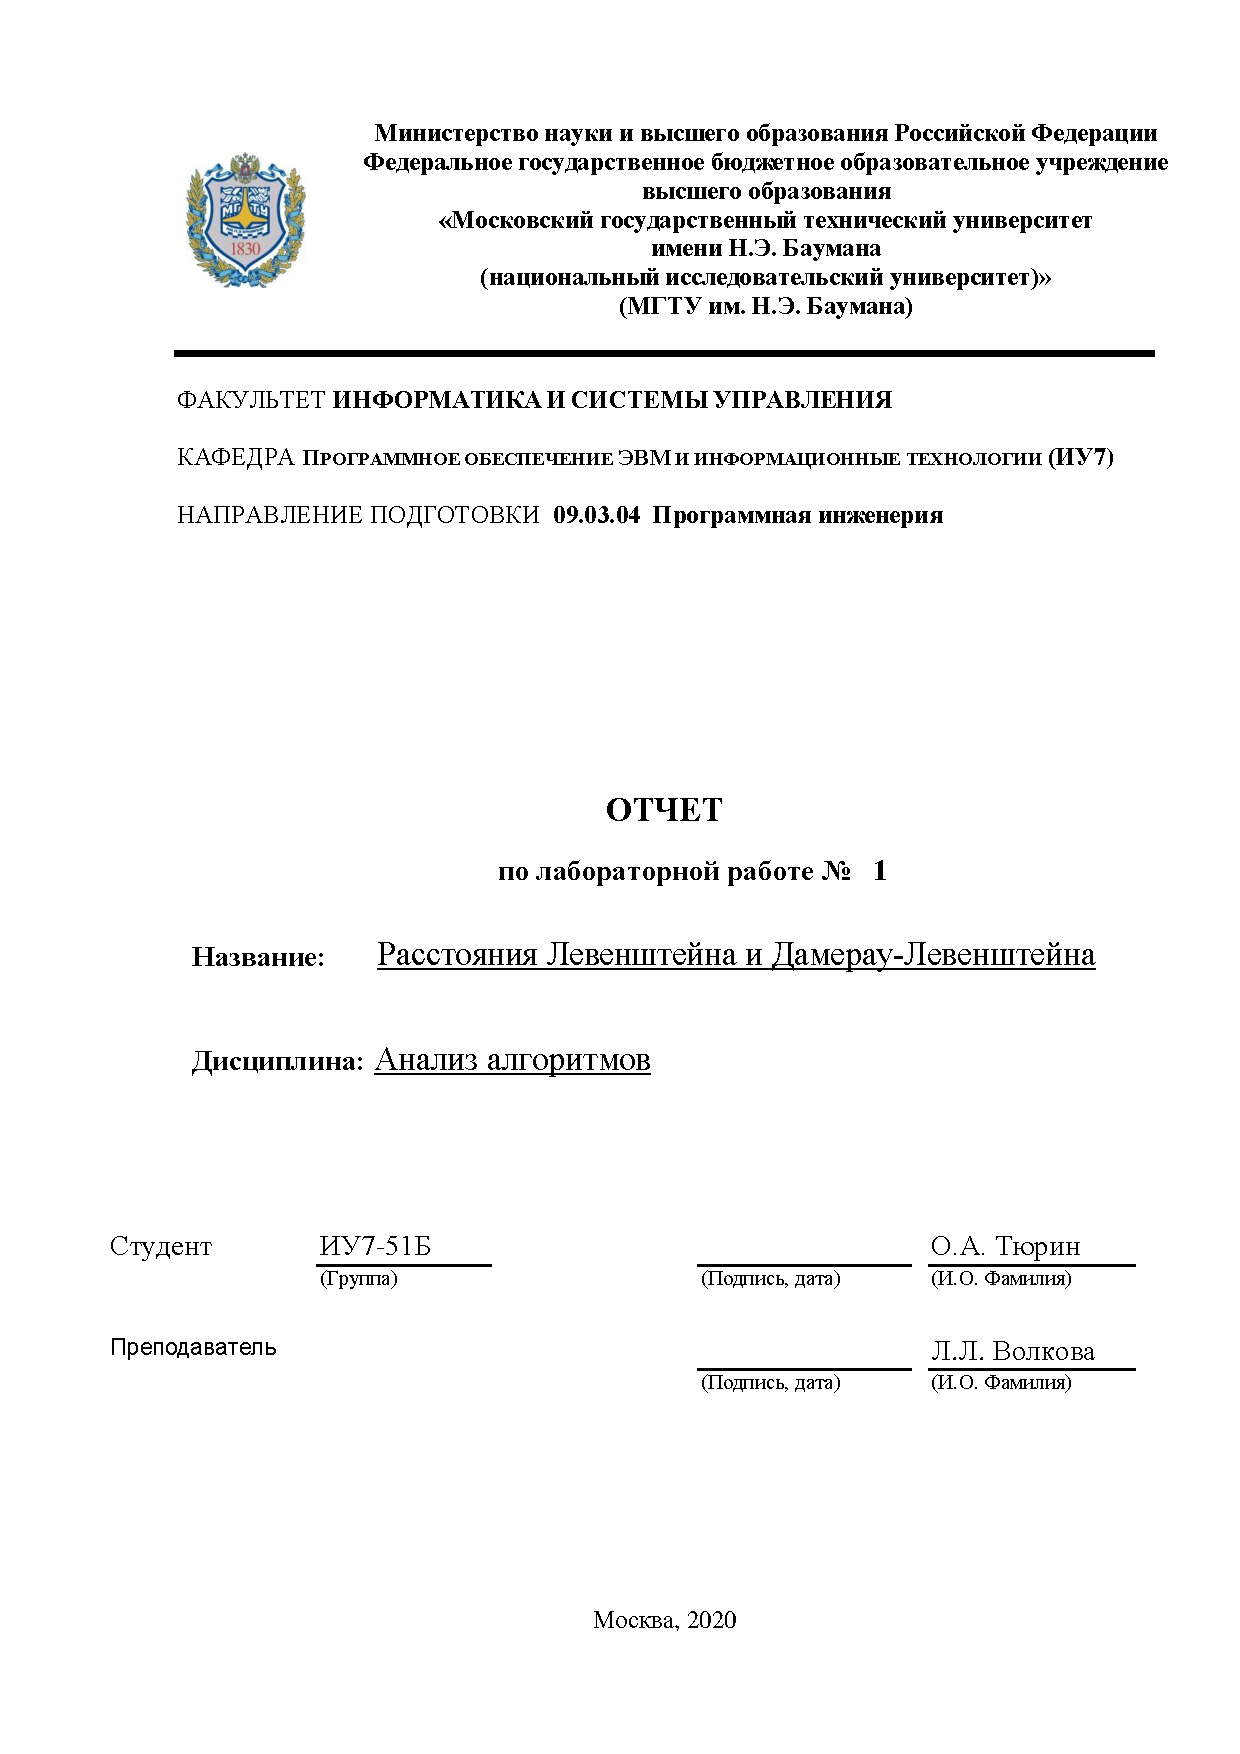
\includegraphics{reportTitle}
		\end{textblock*}
	\end{titlepage}
\hspace{0pt}
\clearpage
%	\begin{titlepage}
%		\centering
%		\Huge Лабораторная работа №1 по курсу \\\textbf{"Анализ алгоритмов"}\\
%		Тема: Расстояния Левенштейна и Дамерау-Левенштейна\\
%		\vspace{\baselineskip}
%		\Large Работу выполнил: Тюрин О.А. ИУ7-51Б\\
%		Преподаватели: Волкова Л.Л.
%		\vfill
%		Москва, 2020 г.		
%	\end{titlepage}
\tableofcontents
\clearpage

\addcontentsline{toc}{section}{Введение}
%//////////////////////////////////////////////////////////////////
\section*{\Huge Введение}
Расстояние Левенштейна (редакционное расстояние) - это минимальное кол-во редакторских операций, которое необходимо для превращения одной строки в другую.\\
\\
Существуют следующие применения редакционных расстояний.\\
1) Поисковики (Google), автоисправление текста.\\
2) Биоинформатика.\\
\\
Задачи для данной ЛР:\\
1) изучение алгоритмов Левенштейна и Дамерау-Левенштейна нахождения расстояния между строками;\\
2) получение практических навыков реализации указанных алгоритмов: двух алгоритмов в матричной версии и одного из алгоритмов в рекурсивной версии;\\
3) сравнительный анализ линейной и рекурсивной реализаций выбранного алгоритма определения расстояния между строками по затрачиваемым ресурсам (времени и памяти);\\
4) эксперементальное подтверждение различий во временной эффективности рекурсивной и нерекурсивной реализаций выбранного алгоритма определения расстояния между строками при помощи разработанного программного обеспечения на материале замеров процессорного времени выполнения реализации на варьирущихся длинах строк;\\
5) описание и обоснование полученных результатов в отчете о выполненной лабораторной работе.\\
\clearpage

\section{Аналитическая часть}
Задача по нахождению расстояния Левенштайна заключается в поиске минимального количества операций с единичным штрафом.\\
\textbf{Вставка (I - Insert)}\\
\textbf{Удаление (D - Delete)}\\
\textbf{Замена (R - Replace)}\\
\textbf{Совпадение (M - Match)}\\
Для превращения одной строки в другую.\\
В алгоритме Далмерау-Левенштайна добавляется ещё одна операция:\\
\textbf{Транспозиция(T)}\\
Все операции, кроме "Совпадения", имеют штраф 1. Операция "Совпадения" имеет штраф 0.
\newpage
\subsection{Описание расстояний и алгоритмов}

\subsubsection{Расстояние Левенштейна, рекурсивное определение расстояния}
Введём понятие D(s1, s2) = минимальному количеству редакторских операций, с помощью которых строка s1 преобразуется в строку s2.
Тогда расстояние Левенштейна можно записать следующим образом:\\
$
D(i, j) = \begin{cases}
	0, i = 0, j = 0 \\
	i, j = 0, i > 0 \\
	j, i = 0, j > 0 \\
	min(D(S_{1}[1, ..., i], S_{2}[1, ..., j - 1]) + 1,\\
	D(S_{1}[1, ..., i - 1], S_{2}[1, ..., j]) + 1,\\
	D(S_{1}[1, ..., i - 1], S_{2}[1, ..., j - 1]) + \\
	\left[
	\begin{gathered}
	0, if S_{1}[i] = S_{2}[j],\\
	1, else
	\end{gathered}
	\right.
\end{cases}
$
Расстояние можно искать рекурсивно по представленной формуле.

\subsubsection{Расстояние Левенштейна, матричное определение расстояния}
Вводится матрица, размерностью $[Len(S_{1}) + 1 \textbf{X} Len(S_{2}) + 1]$\\
Первая строки и столбец матрицы заполняются от 0 до Len(S) (первые 3 пункта системы из предыдущего пункта).\\
\\
\begin{equation*}
A = \left(
\begin{array}{ccccccc}
 & \emptyset & \text{С} & \text{Т} & \text{О} & \text{Л} & \text{Б}\\
\emptyset & 0 & 1 & 2 & 3 & 4 & 5\\
\text{Т} & 1 & & & & & \\ 
\text{Е} & 2 & & & & & \\
\text{Л} & 3 & & & & & \\
\text{О} & 4 & & & & & \\
\end{array}
\right)
\end{equation*}

Далее для нахождения ответа применяется последняя формула из системы, описанной в предыдущем пункте.

\begin{equation*}
A = \left(
\begin{array}{ccccccc}
& \emptyset & \text{С} & \text{Т} & \text{О} & \text{Л} & \text{Б}\\
\emptyset & 0 & 1 & 2 & 3 & 4 & 5\\
\text{Т} & 1 & 1 & 1 & 2 & 3 & 4 \\ 
\text{Е} & 2 & 2 & 2 & 2 & 3 & 4 \\
\text{Л} & 3 & 3 & 3 & 3 & 2 & 3 \\
\text{О} & 4 & 4 & 4 & 3 & 3 & \textbf{3} \\
\end{array}
\right)
\end{equation*}
\\
Ответ в правом нижнем углу.\\
\\
Чтобы определить, какая именно цепочка преобразований привела к ответу представим матрицу как карту высот: нужно спуститься на санках из клетки с ответом в левый верхний угол. В нашем случае:\\
$\textbf{I}$: ТЕЛО $\rightarrow$ СТЕЛО\\
$\textbf{M}$: Т = Т\\
$\textbf{R}$: Е $\rightarrow$ О\\
$\textbf{M}$: Л = Л\\
$\textbf{R}$: О $\rightarrow$ Б\\


\subsubsection{Расстояние Левенштейна, рекурсивное матричное определение расстояния}
Аналогичен алогритму из предыдущего пункта с той лишь разницей, что матрица начинает заполнение "с конца". Вычисляем значение ячейки матрицы только в том случае, если значения там ещё нет (аналогично $\infty$ в алгоритме Дейкстры). Ответ всё так же в правом нижнем углу.

\subsubsection{Алгоритм поиска расстояния Дамерау-Левенштейна}
\qquad Расстояние Дамерау-Левенштейна вычисляется по следующей формуле:
\begin{displaymath}
D(i,j) = \left\{ \begin{array}{ll}
0, & \textrm{$i = 0, j = 0$}\\
i, & \textrm{$j = 0, i > 0$}\\
j, & \textrm{$i = 0, j > 0$}\\
min(\\
D(S_1[i],S_2[j-1])+1,& \textrm{$ j > 0 \quad //I$}\\
D(S_1[i-1], S_2[j]) +1, &\textrm{$i > 0 \quad //D$}\\
D(S_1[i-1], S_2[j-1]) + \\

\left[ \begin{array}{ll}
0, & \textrm{если $\quad S1[i] == S2[j], \quad //M$}\\
1, & \textrm{иначе $\quad //R$}\\
\end{array}\right.\\
D(S_1[i - 2], S_2[j - 2]) + 1 & \textrm{если $i = 1, j = 1,
											S_1[i] = S_2[j - 1],
											S_1[i - 1] = S_2[j]$}\\
)
\end{array} \right.
\end{displaymath}
\subsection{Вывод}
Были рассмотрены алгоритмы нахождения расстояния Левенштейна и нахождения расстояния Дамерау-Левенштейна. Главное отличие - наличие операции транспозиции. 
\clearpage

\section{Конструкторская часть}
\textbf{Требования к вводу:}\\
1) на вход подаются две строки;\\
2) одна и та же буква в разном регистре считается как разный символ.\\
\textbf{Требования к программе:}:\\
1) Две пустые строки являются корректным вводом, который программа должна обработать.
\clearpage
\subsection{Разработка алгоритмов} % Сюда схемы алгоритмов
В данном разделе представлены схемы реализуемых алгоритмов.
Схема рекурсивного алгоритма поиска расстояния Левенштейна представлена на рис. 1
\begin{center}	
	
	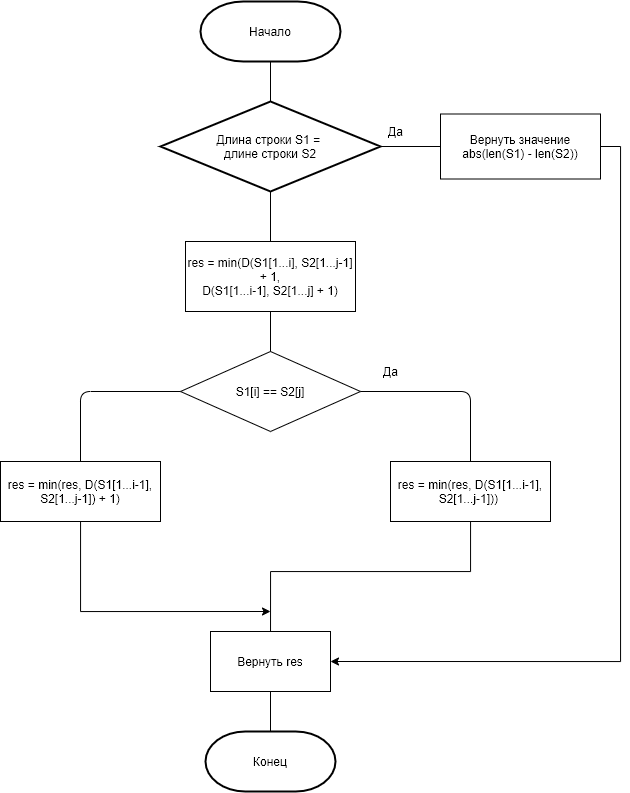
\includegraphics[width=0.9\linewidth]{lev_rec}\\
	\label{formula1} Рис. 1: Cхема рекурсивного алгоритма поиска расстояния Левенштейна
\end{center}
\clearpage
Схема матричной реализации алгоритма поиска расстояния Левенштейна представлена на рис. 2
\begin{center}	
	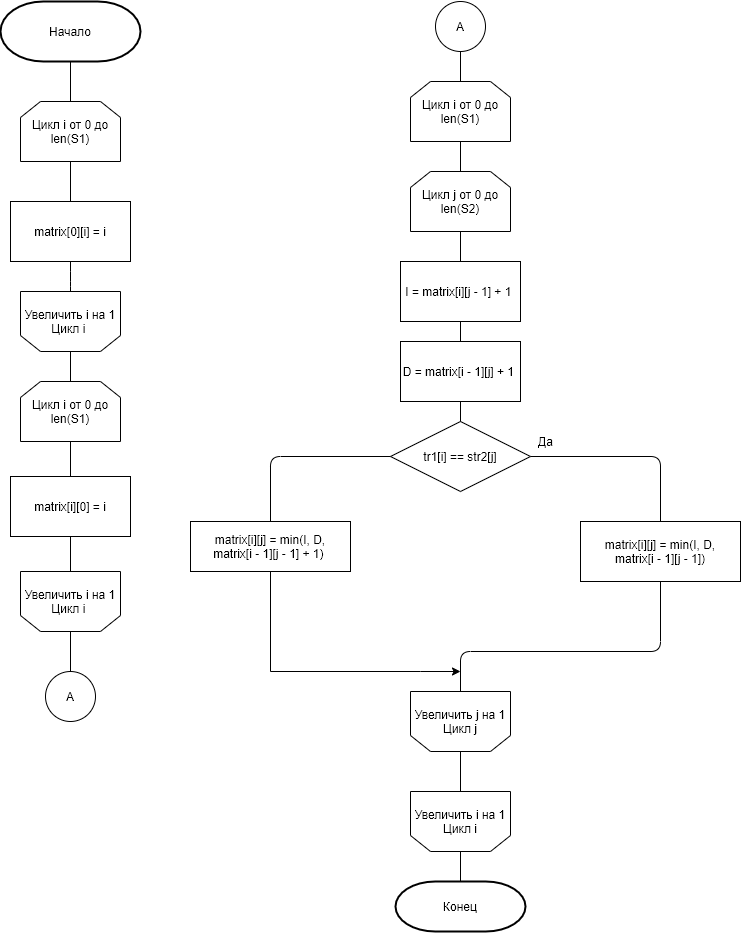
\includegraphics[width=.9\linewidth]{lev_matr}\\
	Рис. 2: Cхема матричной реализации алгоритма поиска расстояния Левенштейна
\end{center}
\clearpage
Схема рекурсивного матричного алгоритма поиска расстояния Левенштейна представлена на рис. 3
\begin{center}
	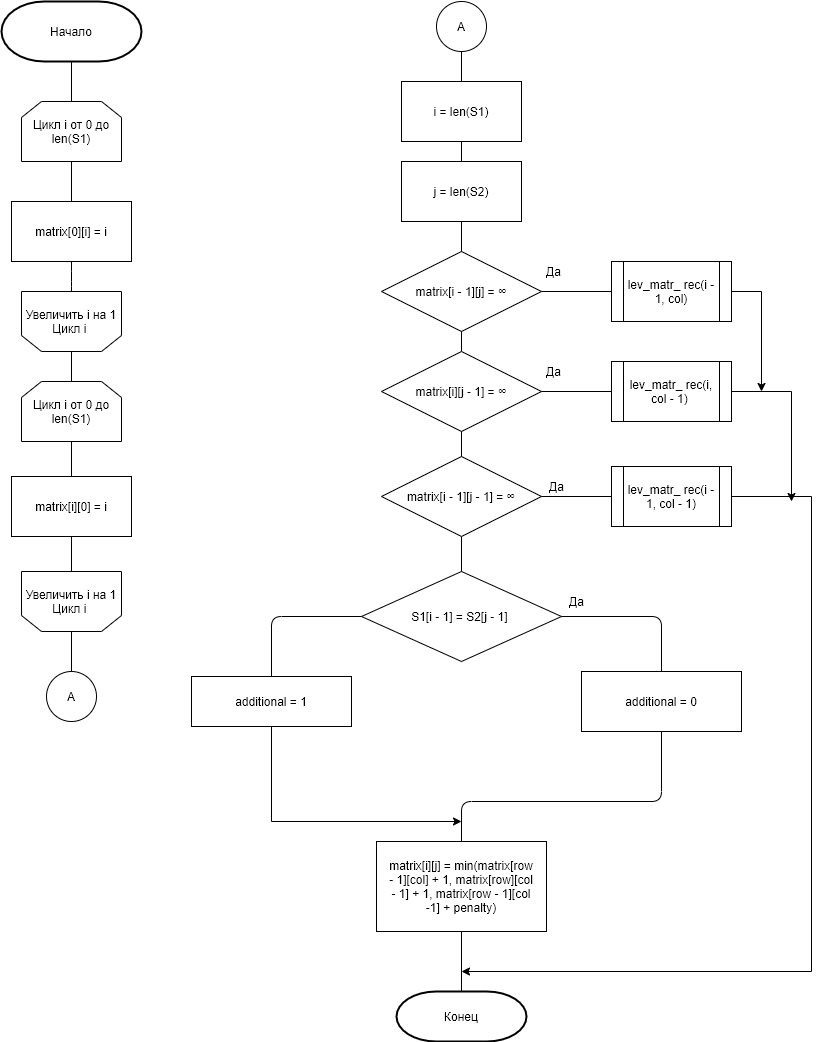
\includegraphics[width=1\linewidth]{lev_matr_rec}\\
	Рис. 3: Cхема рекурсивной матричной реализации алгоритма поиска расстояния Левенштейна
\end{center}
\clearpage
Схема алгоритма поиска расстояния Дамерау-Левенштейна представлена на рис. 4
\begin{center}
	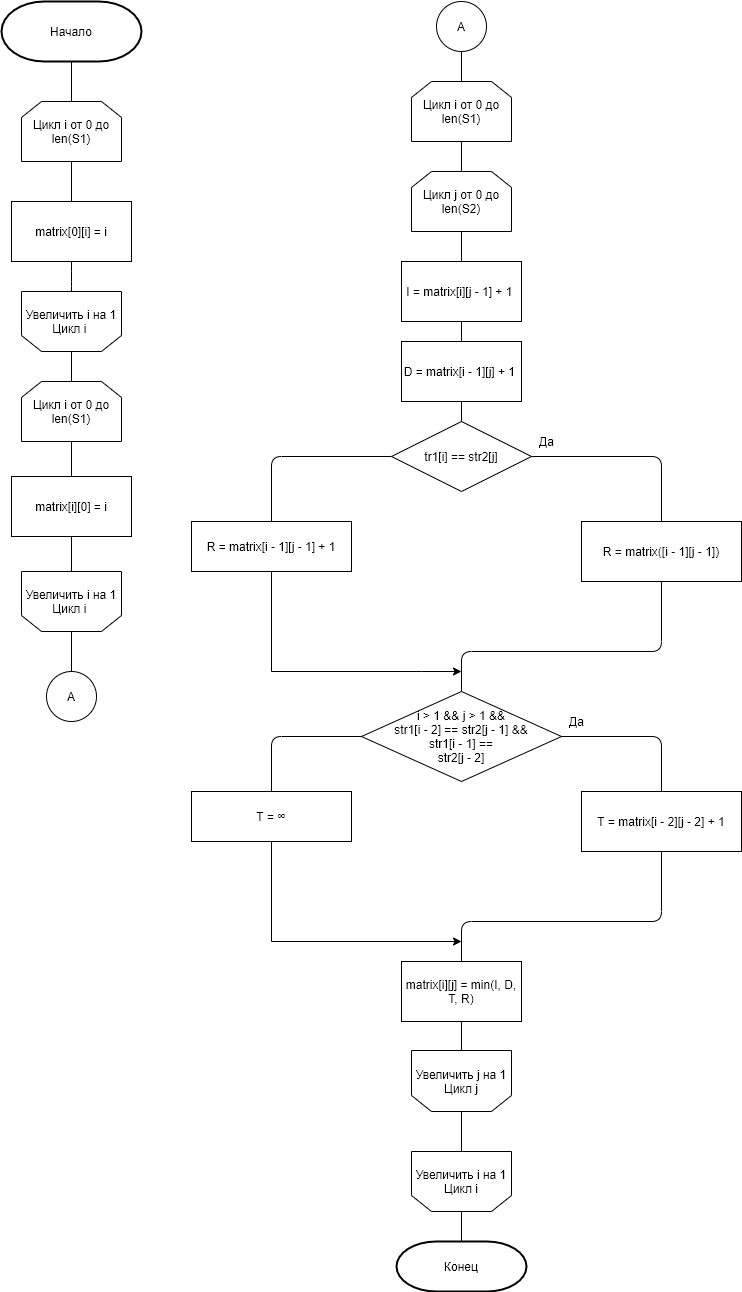
\includegraphics[width=.67\linewidth]{dam_lev}\\
	Рис. 4: Схема алгоритма поиска расстояния Дамерау-Левенштейна
\end{center}
\subsection{Вывод}
\qquad Были рассмотрены и обозначены требования к программе, а также к входным и выходным параметрам в программе. Также были рассмотрены и представлены схемы всех рассматриваемых алгоритмов.
\clearpage

\section{Технологическая часть}
В данном разделе будет описана технологическая часть лабораторной работы: требования к ПО, листинг кода, сравнительный анализ всех алгоритмов.
\subsection{Требования к программному обеспечению}
Входные данные: два слова: str1, str2\\
Выходные данные: редакционное расстояние данных слов, а также матрица решения для матричных реализаций\\
Среда выполнения: Windows 10 x64
\subsection{Средства реализации}
Для выполнения данной лабораторной работы использовался ЯП Python 3.9.0 \\
\subsection{Листинг кода}
В данном разделе будет представлен листинг кода разработанных алгоритмов (листинги 1 - 4).\\

\subsubsection{Рекурсивный алгоритм Левенштейна}
\begin{center}
	Листинг 1: Рекурсивный алгоритм Левенштейна
	\lstinputlisting[language=C++]{lev_rec.py}
\end{center}
\clearpage

\subsubsection{Матричный алгоритм Левенштейна}
\begin{center}
	Листинг 2: Матричный алгоритм Левенштейна
	\lstinputlisting[language=python]{lev_matr.py}
\end{center}

\subsubsection{Рекурсивный матричный алгоритм Левенштейна}
\begin{center}
	Листинг 3: Рекурсивный матричный алгоритм Левенштейна
	\lstinputlisting[language=python]{lev_matr_rec.py}
\end{center}
\clearpage

\subsubsection{Алгоритм Дамерау-Левенштейна}
\begin{center}
	Листинг 4: Алгоритм Дамерау-Левенштейна
	\lstinputlisting[language=python]{dam_lev.py}
\end{center}


\subsection{Сравнительный анализ матричной и рекурсивной реализаций}
\qquad Алгоритмы Левенштейна и Дамерау — Левенштейна не отличаются друг от друга с точки зрения использования памяти.\\
\qquad \textbf{Рассмотрим разницу между рекурсивной и матричной реализациями:}\\
Рекурсивная версия алгоритма работает существенно медленне матричной реализации ввиду многократного вызова функции. На каждый вызов необходимо производить соответствующие операции со стеком. Более того, главным недостатком является - повторное вычисление тех значений, которые были посчитаны на более ранних этапах рекурсии. В матричных реализация будет затрачена дополнительная память на хранение матриц и дополнительных переменных в цикле, однако время работы подобной реализации будет значительно быстрее рекурсивной.
\subsubsection{Теоретический анализ затрачиваемой памяти}
\textbf{Рекурсивная реализация алгоритма Левенштейна}. Для получения конечной оценки затрачиваемой памяти необходимо память, затрачиваемую на единичный вызов функции умножить на максимальную глубину рекурсии, то есть на n + m, где n и m - длины сравниваемых строк s1 и s2 соответственно.
\begin{enumerate}
	\item ссылки на строки s1, s2: (m + n) * sizeof(str),
	\item длины строк: 2 * sizeof(int),
	\item дополнительная переменная внутри алгоритма: sizeof(int)
	\item адрес возврата
\end{enumerate}
memory = (m + n) * ((m + n) * sizeof(str) + 2 * sizeof(int) + 4 bytes)
\\\\
\textbf{Матричная реализация алгоритма Левенштейна}
\begin{enumerate}
	\item строки: sizeof(str) * (n + m)
	\item матрица: sizeof(int) * (n + 1) * (m + 1)
	\item дополнительная переменная внутри алгоритма: sizeof(int)
\end{enumerate}
memory = sizeof(str) * (n + m) + sizeof(int) * (n + 1) * (m + 1) + sizeof(int)
\\\\
\textbf{Рекурсивный матричный алгоритм Левенштейна}. Аналогично обычному рекурсивному алгоритму для получения конечной оценки затрачиваемой памяти необходимо память, затрачиваемую на каждом рекурсивном вызове умножить на максимальную глубину рекурсии.

\begin{enumerate}
	\item строки: sizeof(str) * (n + m)
	\item матрица: sizeof(int) * (n + 1) * (m + 1)
\end{enumerate}
memory = (m + n) * (sizeof(str) * (n + m) + sizeof(int) * (n + 1) * (m + 1))
\\\\
При каждой необходимости предварительного подсчёта значения (рек. вызова)
\begin{enumerate}
	\item передача строки и столбца: 2 * sizeof(int)
	\item дополнительная переменная: sizeof(int)
	\item адрес возврата
\end{enumerate}
memory = (m + n) * (2 * sizeof(int) + sizeof(int) + 4 bytes)
\\\\
\textbf{Матричная реализация алгоритма Дамерау-Левенштейна}
\begin{enumerate}
	\item строки: sizeof(str) * (n + m)
	\item матрица: sizeof(int) * (n + 1) * (m + 1)
	\item дополнительная переменная внутри алгоритма: sizeof(int)
\end{enumerate}
memory = sizeof(str) * (n + m) + sizeof(int) * (n + 1) * (m + 1) + sizeof(int)

\subsection{Интерфейс программы}
При запуске программы пользователя встречает меню выбора реализаций алгоритма:\\
\begin{center}
	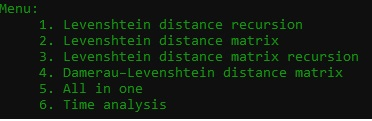
\includegraphics{menu}\\
	Рис.5: Меню программы
\end{center}
После выбора необходимой реализации пользователю предлагают ввести строки s1 и s2. После ввода программа выдаёт результат:\\
\begin{center}
	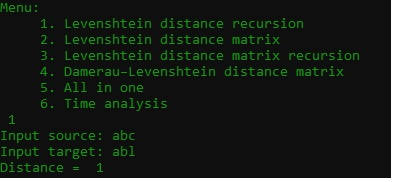
\includegraphics{examp}\\
	Рис.6: Ввод строк и результат работы программы
\end{center}
\subsection{Тестирование}
% описать, какие тесты будут проведены ВСЕ ТЕСТЫ ПРОЙДЕНЫ УСПЕШНО
Тестирование проводилось по методу черного ящика.
При сравнении результатов двух функций использовалась функция random string, которая генерирует случайную строку нужной длины.
\begin{center}
	Листинг 5: Функция random string
	\lstinputlisting[language=C++]{random_string.py}
\end{center}
Листинг 6: Тестирование
	\lstinputlisting[language=C++]{test.py}
Все тесты пройдены успешно
\subsection{Вывод}\\
Были разработаны, протестированы и проанализированы спроектированные алгоритмы: вычисления расстояния Левенштейна рекурсивно, с заполнением матрицы и рекурсивно с заполнением матрицы, а также вычисления расстояния Дамерау-Левенштейна с заполнением матрицы.
\clearpage

\section{Экспериментальная часть}
В данной части работы будут приведены примеры работы программ, а также анализ алгоритмов на основе экспериментальных данных.
\subsection{Примеры работы}
Проверка на пустые строки:
\begin{lstlisting}
	source = ""
	target = ""
	Levenshtein Recursive: 0
	Levenshtein Matrix: 0
	Levenshtein Matrix Recursive: 0
	Damerau Levenshtein: 0
\end{lstlisting}
Проверка на на равенство строк:
\begin{lstlisting}
	source = "abc"
	target = "abc"
	Llevenshtein Recursive: 0
	Levenshtein Matrix: 0
	Levenshtein Matrix Recursive: 0
	Damerau Levenshtein: 0
\end{lstlisting}

Операция удаления:
\begin{lstlisting}
	source = "abc"
	target = "ab"
	Levenshtein Recursive: 1
	Levenshtein Matrix: 1
	Levenshtein Matrix Recursive: 1
	Damerau Levenshtein: 1
\end{lstlisting}

Операция замены:
\begin{lstlisting}
	source = "abf"
	target = "abc"
	Levenshtein Recursive: 1
	Levenshtein Matrix: 1
	Levenshtein Matrix Recursive: 1
	Damerau Levenshtein: 1
\end{lstlisting}

Операция вставки:
\begin{lstlisting}
	source = "ab"
	targer = "abc"
	Levenshtein Recursive: 1
	Levenshtein Matrix: 1
	Levenshtein Matrix Recursive: 1
	Damerau Levenshtein: 1
\end{lstlisting}
\clearpage
Операция перестановки
\begin{lstlisting}
	source = "abc"
	target = "acb"
	Levenshtein Recursive: 2
	Levenshtein Matrix: 2
	Levenshtein Matrix Recursive: 2
	Lamerau Levenshtein: 1
\end{lstlisting}
\subsection{Постановка эксперимента по замеру времени}
Были произведены замеры для строк длиной от 0 до 9.\\
Для каждой размерности было проведено 100 вызовов функции. После чего получившеесся время было поделено на 100. Таким образом было получено аппроксимированное значение времени выполнения функции\\
Результаты замеров процессорного времени:\\
\begin{center}
	Был проведен замер времени работы каждого из алгоритмов.

\begin{center}
	\begin{tabular}{|c c c c c|} 
 	\hline
	len & Lev(R) & Lev(M) & Lev(MR) & DamLev \\ [0.5ex] 
 	\hline\hline
 	3 & 0.00003 & 0.00001 & 0.00001 & 0.00001\\
 	\hline
 	4 &  0.00017  &  0.00001 &  0.00002 & 0.00001\\
 	\hline
	5 & 0.00105 & 0.00002 & 0.00014 & 0.00002\\
	\hline
	6 &  0.00505 & 0.00003 & 0.00004 & 0.00005\\
	\hline
	7 & 0.03235 & 0.00004 & 0.00006 & 0.00006\\
	\hline
	8 & 0.18632 & 0.00006 & 0.00007 & 0.00008\\
	\hline
	9 & 1.39152 & 0.00011 & 0.00024 & 0.00012\\
	\hline
	\end{tabular}
\end{center}

\begin{center}
График 1: Замеры времени работы алгоритмов
	\begin{tikzpicture}
	\begin{axis}
	[ legend pos=north west	,
	xlabel = {Размер строки},
    ylabel = {Время (с)}]
	\addplot [color=blue] coordinates {
		(0, 0)(3, 0.00003) (4,  0.00017) (5, 0.00105) (6, 0.00505) (7, 0.03235) (8, 0.18632) (9, 1.39152)
	};
	\addplot [color=brown] coordinates {
	(0, 0) (3, 0.00001) (4, 0.00001) (5, 0.00002) (6, 0.00003) (7, 0.00004) (8, 0.00006) (9, 0.00011) 
	};
	\addplot [color=black] coordinates {
		(0, 0)(3,  0.00001) (4, 0.00002) (5, 0.00014) (6, 0.00004) (7, 0.00006) (8, 0.00007) (9, 0.00024) 
	};
	\addplot [color=red] coordinates {
		(0, 0)(3,  0.00001) (4, 0.00001) (5, 0.00002) (6, 0.00005) (7, 0.00006) (8, 0.00008 ) (9, 0.00012) 
	};
	\end{axis}
	\end{tikzpicture}
	\\
	Легенда:\\
	Синий цвет - Рекурсивная реализация\\
	Коричневый цвет - Матричная реализация\\
	Чёрный цвет - Рекурсивная матричная реализация\\
	Красный цвет - Алгоритм Дамерау-Левенштейна\\
	
	
\end{center}

\begin{center}
График 2: Замеры времени работы алгоритмов
	\begin{tikzpicture}
	\begin{axis}
	[ legend pos=north west	,
	xlabel = {Размер строки},
    ylabel = {Время (мс)}]
	\addplot [color=brown] coordinates {
	(0, 0) (3, 0.00001) (4, 0.00001) (5, 0.00002) (6, 0.00003) (7, 0.00004) (8, 0.00006) (9, 0.00011) 
	};
	\addplot [color=black] coordinates {
		(0, 0)(3,  0.00001) (4, 0.00002) (5, 0.00004) (6, 0.00006) (7, 0.00010) (8, 0.00014) (9, 0.00024) 
	};
	\addplot [color=red] coordinates {
		(0, 0)(3,  0.00001) (4, 0.00001) (5, 0.00002) (6, 0.00005) (7, 0.00006) (8, 0.00008 ) (9, 0.00012) 
	};
\addlegendentry{Матричный}
\addlegendentry{Рекурсивно-матричный}
\addlegendentry{Дамерау-Левенштейна}
	\end{axis}
	\end{tikzpicture}
\end{center}

\begin{flushleft}
\subsection{Сравнительный анализ на материале экспериментальных данных}
Рекурсивный алгоритм Левенштейна работает дольше итеративных реализаций, время его работы увеличивается в геометрической прогрессии. При увеличении длины строк становится очевидна выигрышность по времени матричного варианта.\\
Рекурсивный алгоритм с заполнением матрицы превосходит простой рекурсивный на аналогичных данных. Алгоритм Дамерау — Левенштейна по времени выполнения сопоставим с алгоритмом Левенштейна. В нём добавлены дополнительные проверки, и по сути он является алгоритмом другого смыслового уровня.\\
По расходу памяти итеративные алгоритмы проигрывают рекурсивному: максимальный размер используемой памяти в них растёт как произведение длин строк, в то время как у рекурсивного алгоритма — как сумма длин строк.
\subsection{Вывод}
Теоретические расчёты подтвердились результатами, полученными на пратике: рекурсивный алгоритм ввиду многократного вызова функции и пересчёта уже известных значений выполняется крайне долго, рекурсивная матричная реализация выполняется быстрее, но всё равно из-за операций со стеком и вызовом самой себя уступает по времени обычной матричной реализации. Алгоритм Дамерау-Левенштейна уступает по времени обычной матричной реализации ввиду дополнительной проверки на перестановку  символов.
\end{flushleft}
\clearpage


\addcontentsline{toc}{section}{Заключение}
%//////////////////////////////////////////////////////////////////
\clearpage
\section*{\Huge Заключение}
\begin{flushleft}
\qquad Цель достигнута и все задачи выполнены.\\
\qquad В ходе работы были изучены алгоритмы поиска расстояния Левенштейна и Дамерау-Левенштейна. Реализованы алгоритмы поиска расстояния Левенштейна с заполнением матрицы, а также реализован рекурсивный алгоритм поиска расстояния Левенштейна. Экспериментально было установлено, что из трех алгоритмов Левенштейна самым медленным является рекурсивный, а самым требовательным по памяти - рекурсивный алгоритм с заполнением матрицы, однако так же было установлено, что за счет ее заполнения не происходит повторных вычислений, что существенно повышает скорость выполнения.
Сравнение матричного алгоритма Левенштейна и Дамерау-Левенштейна показало, что последний работает медленее, в силу того, что на каждой итерации цикла выполняется дополнительная проверка и в случае ее справедливости еще и дополнительные вычисления.\\
\qquad Из написанного выше можно сделать вывод, что именно матричный алгоритм Левенштейна следует использовать при решении задач на нахождение минимального редакционного расстояния.
\end{flushleft}
\clearpage
\begin{thebibliography}{}
	\bibitem{1}  Дж. Макконнелл. Анализ алгоритмов. Активный обучающий подход. – М.: Техносфера, 2017. – 267с
	\bibitem{2}Нечёткий поиск в тексте и словаре [электронный ресурс].Режим доступа:\\ https://habr.com/ru/post/114997/, свободный – (Дата обращения: 5.10.20)
	\bibitem{python}Официальный сайт Python, документация [электронный ресурс]. Режим доступа: https://docs.python.org/3.9, свободный – (Дата обращения: 8.10.20)
\end{thebibliography}

\end{document}